% This is samplepaper.tex, a sample chapter demonstrating the
% LLNCS macro package for Springer Computer Science proceedings;
% Version 2.20 of 2017/10/04
%
\documentclass[runningheads]{llncs}
%
\usepackage{hyperref}
\usepackage[utf8]{inputenc}
\usepackage{float}
\usepackage{todonotes}
%\newcommand{\jk}[1]{\todo[inline]{JK: #1}}
\newcommand{\jk}[1]{}
%\newcommand{\fg}[1]{\todo[inline,backgroundcolor=blue]{FG: #1}}
\newcommand{\fg}[1]{}
\usepackage{graphicx}
\usepackage{cleveref}
\graphicspath{ {images/} }
% Used for displaying a sample figure. If possible, figure files should
% be included in EPS format.
%
% If you use the hyperref package, please uncomment the following line
% to display URLs in blue roman font according to Springer's eBook style:
% \renewcommand\UrlFont{\color{blue}\rmfamily}

\begin{document}
\title{Investigating the Overhead of the REST Protocol when Using Cloud Services for HPC Storage} % Moving Cloud Storage to HPC
%\subtitle{} % Performance Challenges and Opportunities for Cloud Technologies
%
%\titlerunning{Abbreviated paper title}
% If the paper title is too long for the running head, you can set
% an abbreviated paper title here
%
\author{Frank Gadban\inst{1} \and Julian Kunkel\inst{2} \and Thomas Ludwig\inst{3}}
%
\authorrunning{F. Gadban et al.}
% First names are abbreviated in the running head.
% If there are more than two authors, 'et al.' is used.
%
\institute{University of Hamburg, 20146 Hamburg, Germany
\email{frank.gadban@studium.uni-hamburg.de}\\
%\url{https://www.uni-hamburg.de}
\and
Reading University, Reading, UK\\
%\email{j.m.kunkel@reading.ac.uk}
\and
DKRZ, 20146 Hamburg \\
%\email {ludwig@dkrz.de}
}

%
\maketitle       % typeset the header of the contribution
%
\begin{abstract}
With the significant advances in Cloud Computing, it is inevitable to explore the usage of Cloud technology in HPC workflows. While many Cloud vendors offer to move complete HPC workloads into the Cloud, this is limited by the massive demand of computing power alongside storage resources typically required by I/O intensive HPC applications. Eventually, the cost of storing and managing data produced by those applications determines where workloads should run. It is widely believed that HPC hardware and software protocols like MPI yield superior performance and lower resource consumption compared to the HTTP transfer protocol used by RESTful Web Services that are prominent in Cloud execution and Cloud storage. With the advent of enhanced versions of HTTP, it is time to reevaluate the effective usage of cloud-based storage in HPC and their ability to cope with various types of data-intensive workloads. 
In this paper, we investigate the overhead of the REST protocol via HTTP compared to the HPC-native communication protocol MPI when storing and retrieving objects. Albeit we compare the MPI for a communication use case, we can still evaluate the impact of data communication and, therewith, the efficiency of data transfer for data access patterns. We accomplish this by modeling the impact of data transfer using measurable performance metrics. Hence, our contribution is the creation of a performance model based on hardware counters that provide an analytical representation of data transfer over current and future protocols. We validate this model by comparing the results obtained for REST and MPI on two different cluster systems, one equipped with Infiniband and one with Gigabit Ethernet. The evaluation shows that REST can be a viable, performant and resource-efficient solution, in particular for accessing large files. 


\jk{TODO: Später kurze Zusammenfassung of Ergebnissen rein. Wo ist HTTP schlechter als MPI allein}

\keywords{HPC \and Cloud \and Convergence \and HTTP2 \and RESTful APIs \and HTTP3 \and Storage.}
\end{abstract}
%
%
%
\section {Introduction}
High-Performance Computing (HPC) utilizes clusters of powerful and fast interconnected computers that can handle complex and data-intensive computational problems. These systems are managed by batch schedulers \cite{ma2004dynamic} where user jobs are queued to be served based on resource usage and availability and without any visibility or concerns on the costs of running jobs.
Due to various factors, Cloud Computing \,\cite {mell2011nist} gained popularity over the last decade. This has led to the emergence of the \textit{HPC Cloud}, where Cloud providers offer high-end hardware platforms and software environments to run HPC applications.

Previous research in this field focused on moving some post-processing to the cloud or offering cloud-bursting\,\cite{lafayetteexploring}, which means a data center may execute applications on the cloud when the waiting time for job execution in the data center exceeds a certain threshold due to high user demand. However, various limitations introduced by cloud concepts like multi-tenancy and heterogeneity \,\cite{gupta2013improving} alongside the network limitation, the sharing policies in cloud data centers, and virtualization overhead \,\cite{performanceAnalysisHPCinCloud} diminish the performance of tightly coupled HPC applications \,\cite{evangelinos2008cloud}.

Due to its simplicity, reliability, flexibility, and consistency, HTTP is the de facto standard for accessing object storage like Amazon S3 \cite{awsS3Url}, OpenStack Swift, and EMC Atmos. A large number of Scale-Out-File Systems like Ceph and QuoByte offer a REST gateway, largely compatible with S3 or Swift interfaces, for data access and manipulation. A wide adoption of cloud storage in HPC requires the evaluation of  the suitability of using HTTP in the HPC environment as an alternative to HPC-native communication protocols like MPI.
Many prerequisites must be fulfilled to consider HTTP as an alternative to classic HPC data access, transfer, and manipulation protocols. These protocols provide low-latency, high throughput, high availability, highly parallel I/O, and high-scalability \cite{Devresse}. 

In this work, we provide first a detailed examination of the HTTP protocol and its performance in terms of latency and throughput under different conditions for accessing remote data. Secondly, we elaborate on an analytic performance model for data transfer over several protocols, this model allows us to compare current and future protocols in a common framework and will help us predict protocol performance in different hardware environments. We perform several benchmarks comparing MPI to HTTP and use our model to validate the obtained results. Finally, and based on the evaluation, we pinpoint the cause of the HTTP overhead and find that TCP is not the ideal transport protocol for HTTP and that new versions of the HTTP protocol, like HTTP3 which uses UDP, might accelerate the usage of cloud storage in HPC.
The structure of this paper is as follows: \Cref{sec:related} represents the related work. \Cref{sec:methodology} describes the test scenarios and defines the relevant metrics that will be addressed using our benchmarks. \Cref{sec:experiments} describes the experimental procedure, the used systems, and the methodology of the evaluation conducted in this work. \Cref{sec:evaluation} analyzes the obtained results. The last section summarizes our findings.


\section {Related Work} \label{sec:related}

In the world of HPC, computational performance has long exceeded the performance of the traditional file-centric storage systems since the POSIX file system interface was hardly suitable for data management on supercomputers\cite{zadok2017posix}.
Many workarounds to address this issue were proposed, some of them tried to introduce evolved I/O algorithms in MPI, like Data aggregation/sieving in ROMIO,\,\cite{datasievingromio} or to implement different data organizations on the back-end storage, like PLFS\,\cite{bent2009plfs} or to introduce richer data formats for example HDF5, NetCDF\,\cite{hdf5}.

Eventually and although a file represents a convenient way to store the data, the ideal concept for scientific computing/HPC would be rather the use of a data object model\cite{liu2018evaluation} where all levels of metadata are encapsulated. 

Object storage organizes information into containers of flexible sizes, referred to as objects. Each object includes the data itself as well as its associated metadata and has a globally unique identifier.
Objects are often accessed directly from the client application, usually using a RESTful API\,\cite{richardson2008restful}.
As such, any comprehensive performance study of an object storage system should take into consideration the latency introduced by a RESTful system.

Many researchers have tried to solve data transfer issues through HTTP; some\,\cite{forest} proposed encapsulating TCP data in UDP payloads, others\,\cite {Devresse} proposed a dynamic connection pool implemented by using the HTTP Keep-Alive feature to maximize the usage of open TCP connections and minimize the effect of the TCP slow start. Intel\textsuperscript \textregistered  is marketing DAOS\,\cite{DAOS} as the ultimate Open Source Object Store, nonetheless with a high vendor Lock-in potential since the promised performance can only be achieved on its own proprietary Optane\,\cite{Optane} storage Hardware.
Since Infiniband \cite{Infiniband} is one of the most commonly used interconnects in HPC, the performance of IP over Infiniband \cite{bortolotti2011comparison,grant2010study} has been thoroughly studied, however, the performance of HTTP over IP over IB did not get much attention. Our approach to model and analyze the viability of HTTP over Infiniband using performance counters is explained in the next section.



\section {Methodology} \label{sec:methodology}
The two major efficiency indicators addressed in our study are latency and throughput.

The hardware components, their interconnection, and the software stack available to HPC applications are usually trimmed for performance compared to the ones serving common web applications. Performance of HTTP between geographically dispersed nodes is the subject of research \cite{tcpperfprediction}. To our knowledge, few tried to assess the Performance of a REST Service inside HPC, i.e., within a high-performance network. This is why we introduce a modeling approach, based on performance counters, then we perform an evaluation on a testbed, consisting of a content server and a client application consuming the content. Our benchmark for storage access emulates a best-case scenario (HTTP GET Operation / Read Only Scenario from a "remote" Storage Server) because we only want to test the viability and base performance of REST/HTTP as an enabling technology for an object-store. The model with the performance counters can nevertheless be extended to assess and measure the resource consumption of different object storage implementations. The tools and the accomplished tests will be extensively described in Section 4. To identify the major factors impacting the performance, we vary the underlying hardware and the connection mechanism (Ethernet, Infiniband, RDMA) between the server and the client. Finally, to validate our model, we compare its predictions with the experimentally observed values.

\subsection{Performance Model}
To define our performance model, many metrics are to be considered, which depict the used hardware (CPU, Bandwidth ...), the software stack, and the network protocol in use. Alongside the standard network metrics, we focus on hardware counters of the CPU namely the number of required CPU cycles to identify the processing cost of a data transfer and the L3 evicted memory, this can be used further to check the memory efficiency of the different implementations. In a first step, we consider TCP as a transport protocol, however, the model is later extended in Section 5 to cover MPI. The metrics involved can be summarized as follows.

\textit{Fixed system parameters:}
\begin{itemize}
\item R: CPU clock rate in Hz
\item rtt: round trip time
\item mtu: maximum transfer unit
\item mss: maximum segment size, transmission protocol dependent (see \cref{eq:net-tp})
\item mem\_tp: the memory throughput, i.e., the speed of data eviction from L3 to the main memory; influenced by the speed of the different caches
\item eBW \cite{chang1995effective}: is the effective bandwidth between client and server, which is the minimum bandwidth of all the hardware components between them (memory throughput, PCI Bus, network interfaces...)
\end{itemize}

\textit{Experiment-specific configurations and results:}
\begin{itemize}
\item Obj\_size: file size transferred from the server to be read by the client.
\item Nreq: number of requests achieved in 60 sec
\item Ncon: number of open connections kept
\item Nthr: number of CPU threads executing the benchmark on the client.
\end{itemize}

\textit{Observable metrics (e.g., using Likwid):}
\begin{itemize}
\item CUC: number of unhalted cycles on each core %a.k.a. CPU\_CLK\_UNHALTED\_CORE, CUCs and CUCc are for the server and client respectively.
\item L3EV:amount of data volume loaded and evicted from/to L3 from the perspective of CPU cores, i.e. the data flowing through L3\cite{l3explainedlik,intel-l3}, L3EVs and L3EVc are for server and client respectively.
\item PLR: the packet loss rate, which is theoretically proportional to the number of parallel connections. 
\end{itemize}

In our preliminary model t(request) is the time starting from the sending of the first byte of the request to the time the complete response is received, and can be calculated as follows:
\begin{equation}
t(request) = t(client) + t(network) + t(server)
\end{equation}
 where t(client), t(network), t(server) are the time fractions needed by the client, network and server respectively to accomplish the request:
\begin{equation}
t(client) = t(compute) + t(memory) + t(cpu\_client\_busy)
\end{equation}

\begin{equation}
t(server) = t(compute) + t(memory) + t(cpu\_server\_busy) + t(pending)
\end{equation}

As a rough estimation of the network throughput when using the TCP protocol, and based on the Mathis et.al. formula\,\cite{predictability}, while presuming that the TCP window is optimally configured, we can safely assume that:
\begin{equation}
net\_tp= \min\{\frac{mss\cdot C}{RTT \cdot \sqrt{PLR}}, eBW\}
\label{eq:net-tp}
\end{equation}
where C=1 and mss = mtu-40 in case of Ethernet.
From this we can calculate t\_net:
\begin{equation}
 t\_net=Obj\_size / net\_tp + t\_queuing
\end{equation}
For the sake of simplicity, we suppose that the routing devices between the nodes don’t add any latency and as such we can neglect t\_queuing
The execution time t(compute) can then be defined as:
\begin{equation}
t(compute) = CUC /R
\end{equation}
t(memory) is the time to traverse the different memory caches, usually narrowed down to:
\begin{equation}
t(memory)=L3EV/mem\_tp
\end{equation}

Putting it all together, and in the case of intra-node communication, we can safely assume that:
\begin{equation}
t(request)=\frac{CUCs}{Rs}+\frac{L3EVs}{mem\_tp}+\frac{CUCc}{Rc}+\frac{L3EVc}{mem\_tp}+\frac{Obj\_size}{net\_tp}
\end{equation}
Generalizing a bit further, we end up with :
\begin{equation}
\label{eq:model}
t(request)=\alpha\cdot rtt+\beta_1\cdot\frac{CUCs}{Rs}+\beta_2\cdot\frac{L3EVs}{mem\_tp}+\beta_3\cdot\frac{CUCc}{Rc}+\beta_4\cdot\frac{L3EVc}{mem\_tp}+\beta_5\cdot\frac{Obj\_size}{net\_tp}
\end{equation}

Where $\alpha$ is a weighting factor ( 0 $\leq$ $\alpha$ $<$ 1 ) \cite{rfc6298}, $\beta_i$ are platform and protocol dependent factors to be evaluated in a later section.
As such, many factors can influence the above starting from the application delivering the content which affects server CPU and memory usage, those metrics are also affected by the type of client consuming the data as well as by the networking protocol in use and the path traversed by the data. In the following sections, we validate this model while comparing the performance of HTTP over different types of hardware and connection protocols.

\section{Experiments}
\label{sec:experiments}

The tests were performed on two different hardware platforms: the first is the WR Cluster, a small test system available at the University of Hamburg, the second is the Mistral supercomputer\,\cite{mistral}, the HPC system for earth-system research provided at the German Climate Computing Center (DKRZ).


\subsection{Test Environments}
The nodes of the WR Cluster are equipped with two Intel Xeon 5650 processors each offering 6 cores. Hyper-threading is enabled on this cluster and, thus, 24 logical processors are visible in Linux. Those processors operate at a nominal frequency of 2.66GHz and utilize three memory channels.
The supercomputer Mistral \cite{mistral} provides 3000 compute nodes each equipped with an FDR Infiniband interconnect and a Lustre storage system with 54 PByte capacity distributed across two File systems. The nodes used for the testing are equipped with two Intel Broadwell processors (E5-2680 @2.5 GHz).


\subsection{Benchmark and Analysis Tools}\label{subsec:benchmark1}

The RESTful API is the typical way to realize access to object storage, and as such the tools used in this article were preliminary developed to assess HTTP performance.
The first experiment checks the latency introduced by a simple web server serving static files, the setup, shown in \cref{fig:wrk2bench}, consists of the lighttpd web server \cite{lighttpd} hosting files of different sizes. These files are placed initially in the in-memory file system (tmpfs) to minimize any storage-related overhead such as disk drive access time. The tests are accomplished using the wrk2 tool \cite{wrk2URL} which is a typical HTTP load testing tool. To avoid Coordinated Omission \cite{wrk2URL}, wrk2 measures response latency from the time the transmission should have occurred - according to the constant throughput configured for the run- to the moment it was received.

\begin{figure}[H]
\centering
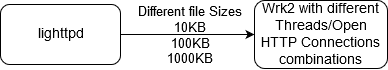
\includegraphics[width=.6\linewidth]{wrk2bench.png}
\caption{A simplified overview of the Benchmark Setup}
\label{fig:wrk2bench}
\end{figure}
In the analysis, we vary the number of threads and the number of HTTP connections kept open while trying to keep a steady rate of 2000 requests/second for 60 seconds for each file size.

\subsection{Latency}\label{subsec:latency}
The diagrams in \cref{fig:latency-to-oc-1000,fig:latency-to-oc-100} show the obtained latency distributions:
\jk{Die Bilder kann man nicht lesen. Text ist einfach zu klein. ca. +80-100\%}
\jk{Immer noch zu klein}
\fg{und nun?}
\begin{figure}[H]
    \centering
    \begin{minipage}{0.49\textwidth}
        \centering
        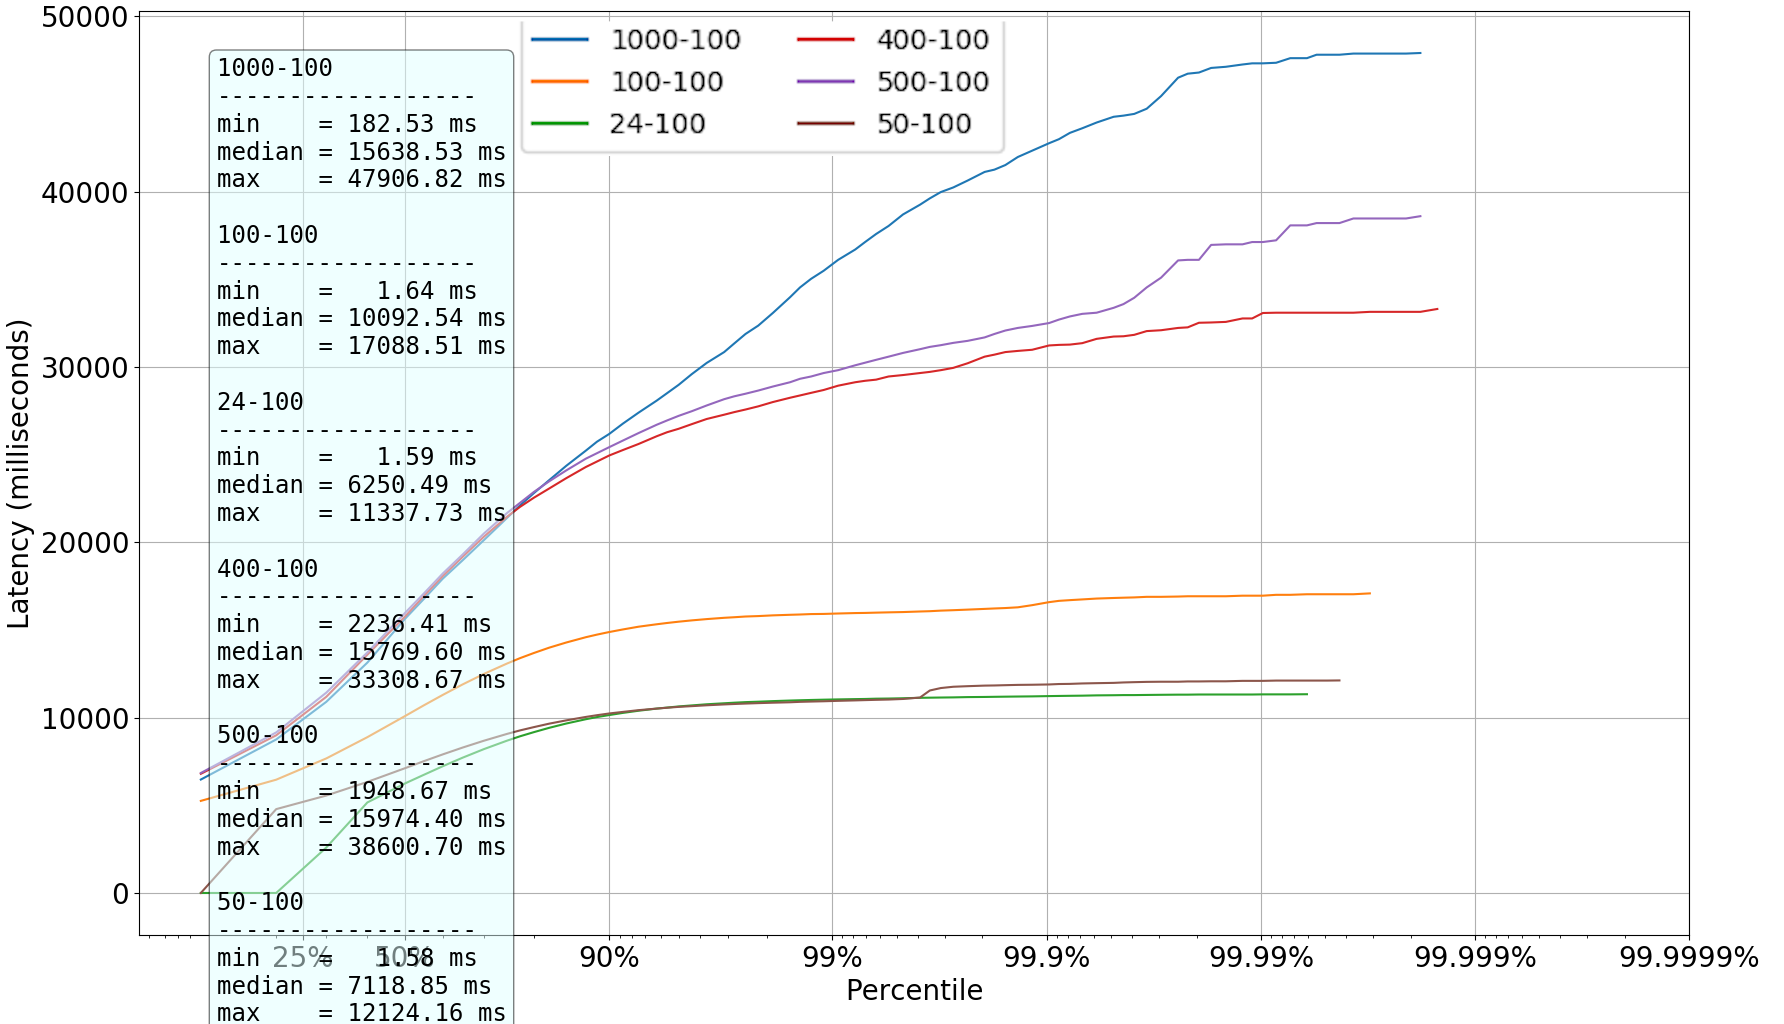
\includegraphics[width=1\textwidth]{plotfile100.png}
        \caption{Latency variation in relation to open connections for a file of size 100\,KB}
			\label {fig:latency-to-oc-100}

    \end{minipage}\hfill
    \begin{minipage}{0.49\textwidth}
        \centering
        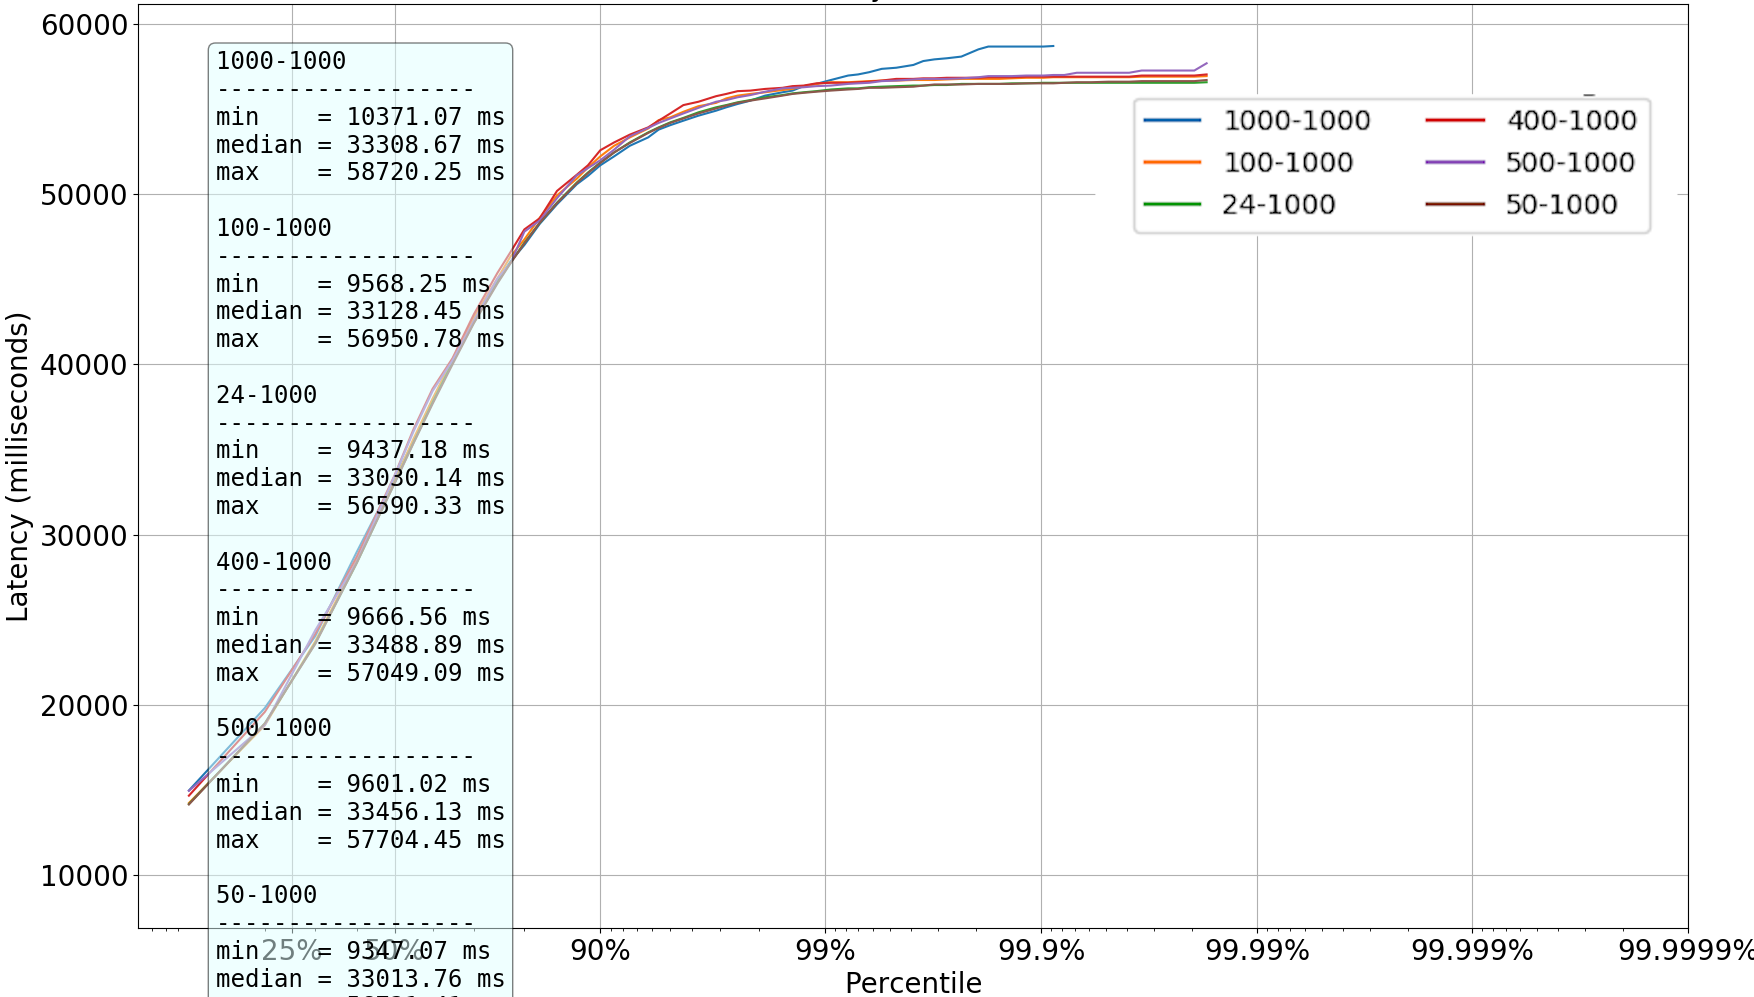
\includegraphics[width=1\textwidth]{plotfile1000.png}
        \caption{Latency variation in relation to open connections for a file of size 1000\,KB}
	   \label {fig:latency-to-oc-1000}
    \end{minipage}
\end{figure}

\begin{figure}
    \centering
    \begin{minipage}{0.49\textwidth}
        \centering
        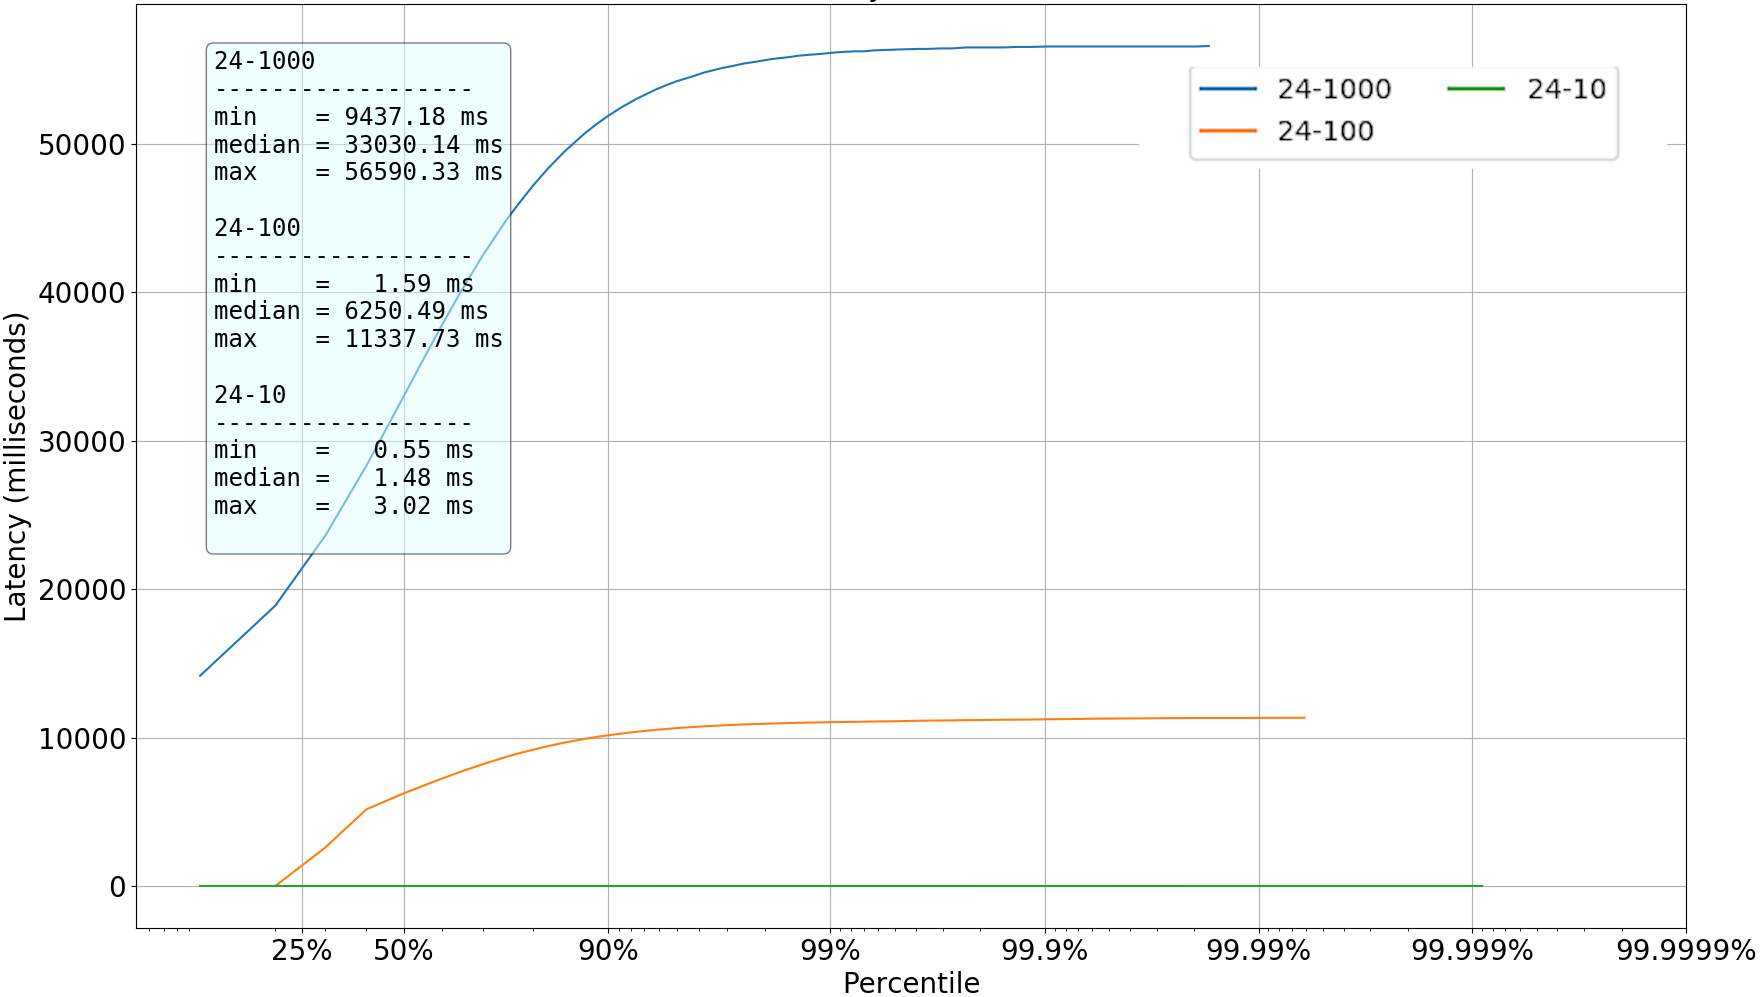
\includegraphics[width=1\textwidth]{plotcon24.png}
        \caption{Latency Variation in relation to file size for 24 open connections}
		\label {fig:latency-to-size-24}
    \end{minipage}\hfill
    \begin{minipage}{0.49\textwidth}
        \centering
        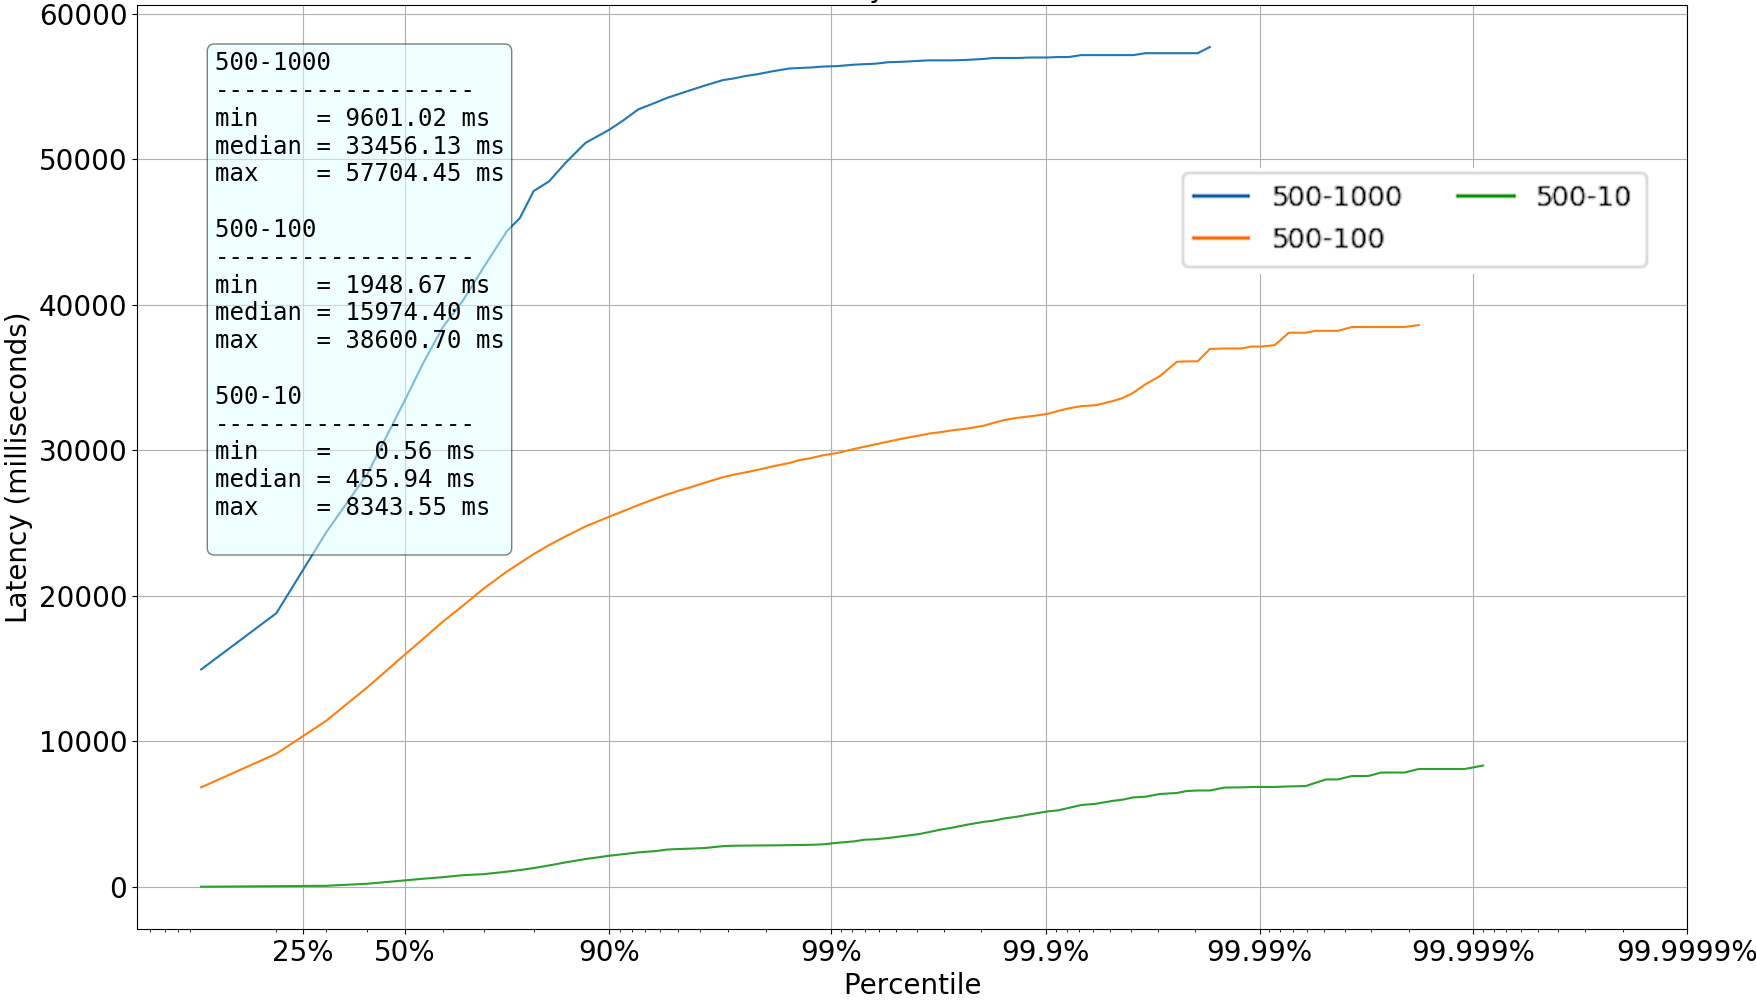
\includegraphics[width=1\textwidth]{plotcon500.png}
        \caption{Latency Variation in relation to file size for 500 open connections}
		\label {fig:latency-to-size-500}
    \end{minipage}
\end{figure}
\textbf{Observations and interpretation:}
\begin{itemize}
  \item Latency does not depend on the duration of the experiment moreover it linearly increases with the number of open connections (see \Cref{fig:latency-to-oc-100} ). The higher the number of connections kept open, the higher is the chance of packet loss leading to the activation of TCP flow control mechanism and eventual data retransmission which in turn cause the increase in latency, this is especially true for small file sizes however when the file size grows beyond a certain limit, the number of connections will become irrelevant to the introduced latency (see \Cref{fig:latency-to-oc-1000}). 
  \item As shown in fig.\ref{fig:latency-to-size-24}, for small file size, we observe a latency divergence in particular in the 99 percentile area
for bigger file size, we noticed in the case of the 100\,KB, the desired request rate of 2000 req/s is not met due to the limitation of the underlying network infrastructure ( 1Gb/s ~ 125 MB/s)
  \item It is interesting to note that, in relation to file size (fig.\ref{fig:latency-to-size-24}) larger files lead to higher memory and network latencies in a way that they can saturate the server’s network bandwidth, lowering throughput (see \Cref{fig:latency-to-oc-1000}). Therefore,  for  serving  large files,  high  network  bandwidth  is  more  important  than compute resources. On the other hand, increasing the number of open Connections (fig.\ref{fig:latency-to-size-500}) will trigger TCP's congestion mechanism and such they will be competing for the same bandwidth. Increasing the file size as well will cause the Open Connections to lose packets and get stuck waiting for retransmissions.
\end{itemize}
A similar latency distribution is observed when the tests are conducted on the same machine, thus using the optimized\cite{linuxkernelcommit} loopback interface, where theoretically the network does not pose any throughput bottleneck (iperf \cite{iperf} result~20 Gbs). However the maximal throughput achieved is 500MB/s, this is mainly due to the fact that the server and the client were competing on the same resource pool since wrk2 is started with 24 threads (the max for each node).

From these experiments, we learn that to optimize the throughput, the web requests should not be using different open connections but rather use one or a relatively small number of open Connections and label the web requests accordingly, which is commonly known as HTTP multiplexing \,\cite{SMUX}, where, using the same TCP connection, multiple HTTP requests are divided into frames, assigned a unique ID called stream ID and then sent asynchronously, the server receives the frames and arranges them according to their stream ID and also responds asynchronously; same arrangement process happens at the client side allowing to achieve maximum parallelism.


\subsection{Throughput}
We consider throughput in terms of the number of requests and the effective network bandwidth. The network throughput of our system is calculated as follow:
\[Throughput=\frac{Nreq \cdot Obj\_size}{time}\]
In our tests, the benchmark ran for a time of 60 seconds, and as such comparing the achievable throughput for the different Connections/Threads combinations yields to comparing the achieved number of requests. \Cref{fig:throughput-to-size} shows that, in the case of inter-node communication, an increase in the number of Open Connections will increase the throughput, on the other side, an increase in the number of threads yields the same effect. However, for file sizes above 1 MB, the influence becomes negligible not to mention that the increase in the number of Threads/Open connections increases the congestion/loss rate causing the benchmark to return different errors.
\begin{figure}
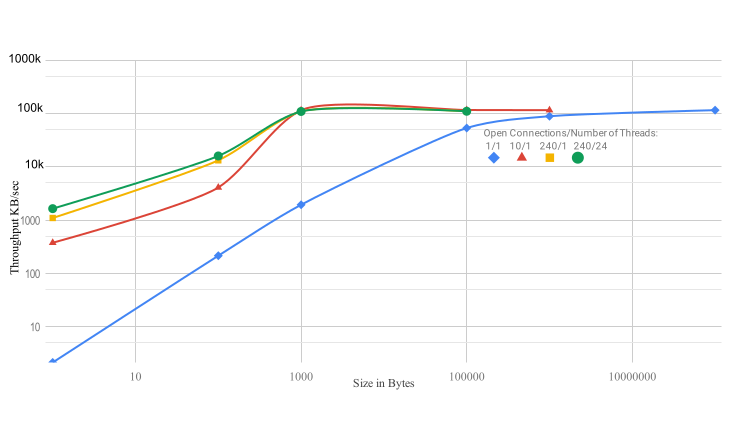
\includegraphics[width=1.0\textwidth]{throughput-to-size.png}
\caption{Throughput in KB/sec related to object size for different combinations of Open Connections/Threads.}
\label{fig:throughput-to-size}
\end{figure}

\subsection{Resource Usage Measurements}

In addition to the latency diagrams and the findings gained from them, another point to consider is the efficiency of the IO itself, this is why we measure the Memory and CPU usage needed to achieve a certain throughput. To accomplish this, likwid-perfctr\,\cite{likwid} is used. It uses the Linux ‘msr’ module to access the model specific registers stored in /dev/cpu/*/msr (which contain hardware performance counters), and calculates performance metrics, FLOPS, bandwidth, etc, based on the event counts collected over the runtime of the application process.
The conducted experiment is similar to Section 4.2, however, this time we are using wrk\cite{wrkURL} without specifying a maximum req/s rate, for 1 minute, during this time Likwid is recording the CPU performance counters which are relevant in this scenario. The server application is pinned to one core using Likwid, the same is done on the client side, As wrk tests are performed using only 1 thread, this doesn’t impose a performance limitations and ensures that the process is run on the first physical core and not migrated between cores which may lead to overhead. 

CPU consumption is recorded, CPU\_CLK\_UNHALTED\_CORE is the metric provided by Likwid that represents the number of clock ticks needed by the CPU to do some reasonable work. The instructions required to accomplish one request - by the server as well as by the client - seems to be linear with the file size, as shown in \Cref{fig:cuc-to-size}. To note here that the server seems to be consuming more CPU cycles as the client to deliver a request, which might be because we are using the lighttpd web server without modifying the default configuration. Note also that over a certain file size limit, the number of timeouts and socket errors increases since we are approaching the maximum throughput that can be achieved by the system.

\begin{figure}
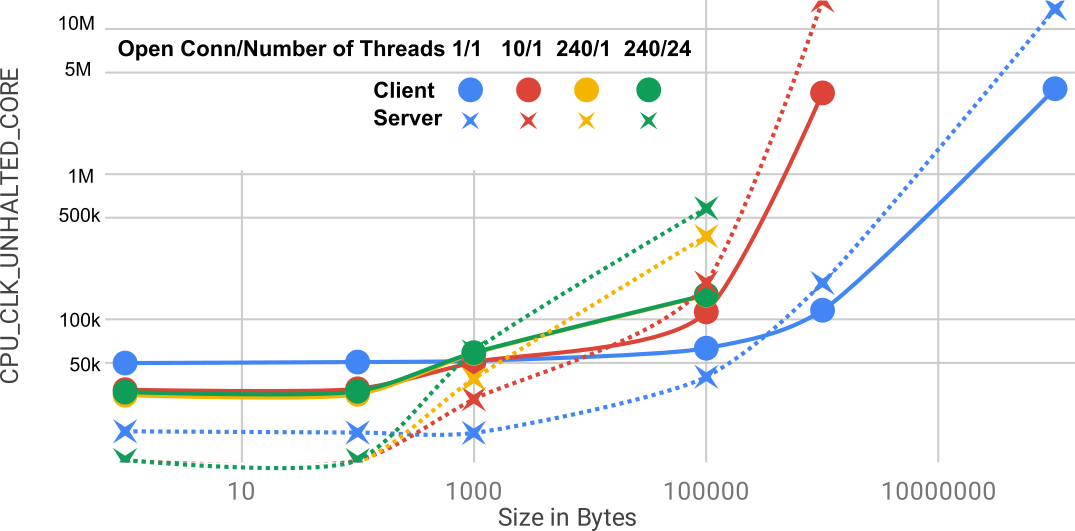
\includegraphics[width=\textwidth]{cuc-to-size.png}
\caption{CPU usage for the client and server related to size, for different Open Connections/Threads combinations}
\label{fig:cuc-to-size}
\end{figure}



\begin{figure}
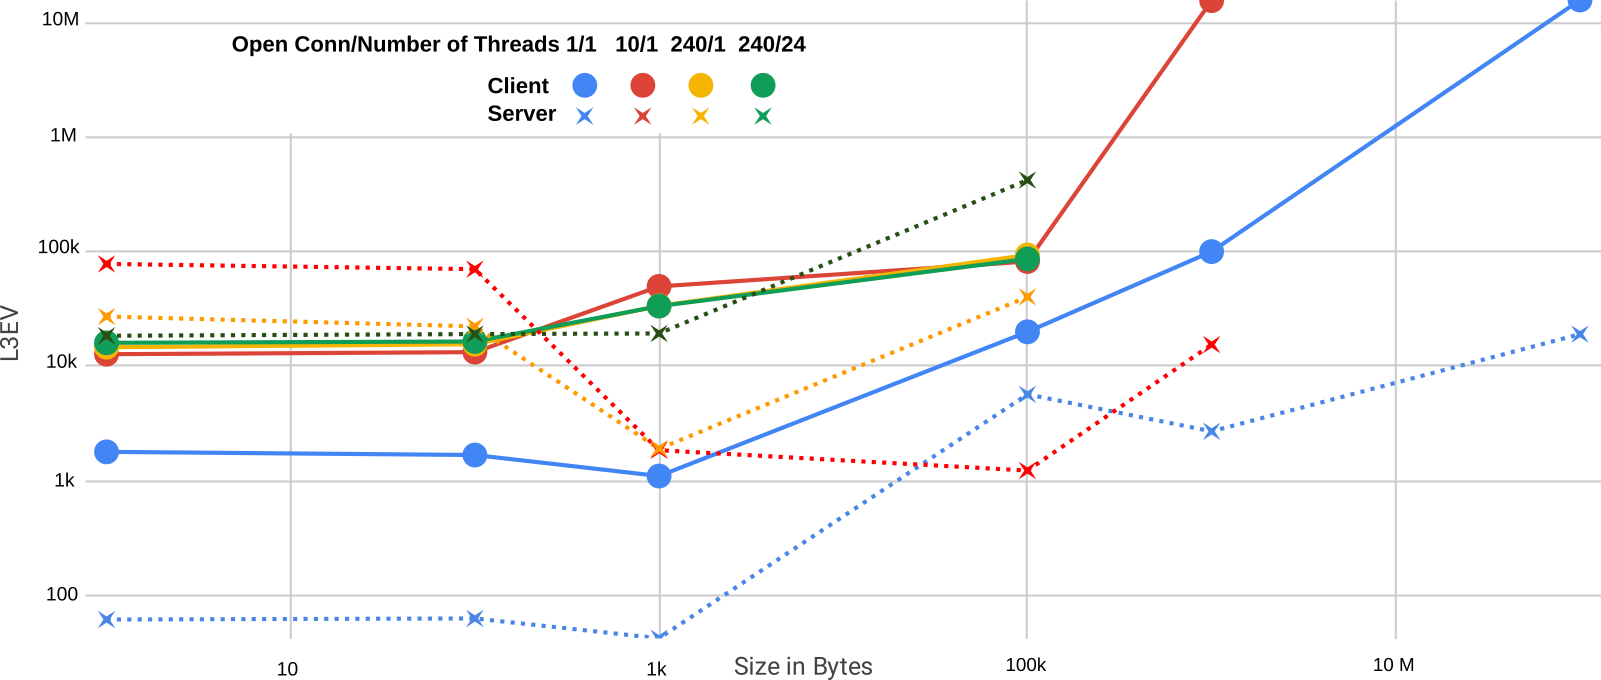
\includegraphics[width=\textwidth]{l3ev-to-size.png}
\caption{L3 evicted volume for the client and server related to size, for different Open Connections/Threads combinations}
\label{fig:l3ev-to-size}
\end{figure}

Regarding memory utilization: Basically, when reading a file (represented by HTTP response), the client needs to store the data received in memory. If the file size exceeds the size of the CPU cache, we expect that data is evicted to main memory, which is measured in L3 cache evictions. This metric is recorded using Likwid and shown in \Cref{fig:l3ev-to-size}. Basically, we can see that even for 100 MB files only 10 MB of data is evicted on the client. There is no eviction on the server because it sends the data directly to the client. This is an indication that zero-copy \cite{zerocopy} is in use on the client and the network interface card offloads the processing of TCP/IP. This allows  the network card to store the data directly into the target memory location. Generally, with zero-copy, the application requests the kernel to copy the data directly from a file descriptor to the socket bypassing the copy in user mode buffer and, therefore, reducing the number of context switches between kernel and user mode.


Furthermore, when data does not fit in the processor L3 caches (12 MB), the evicted data, i.e., the data passed to memory increases significantly causing a performance drop, curiously the rate of increase (slope) of the client evicted memory is greater than on the server, leading us to another interesting conclusion, namely that while most studies focused on optimizing the server-side, it might be the client-side that needs to be addressed.

\subsection{REST vs. MPI}\label{subsec:tcpib}

As found in the previous tests, the available bandwidth plays an important role in determining the latency and the throughput being achieved.The following Tests are achieved on Mistral where Infiniband\,\cite{Infiniband} is available
Our next step is to compare the REST protocol with an established data transfer method in the HPC world, namely the Message Passing Interface MPI\,\cite{MPI}.

To achieve this we launch the same tools used above (likwid+lighttpd) on one node and (likwid+wrk) on another while varying the file size in a power of 2, and recording the different metrics, the transfer takes place over the Infiniband interface.
Then we launch the OSU Micro Benchmark\,\cite{osumicrobenchmark} alongside with likwid on two nodes using the same file sizes and record the same metrics. The OSU tests are executed over Infiniband, the first time by using RDMA and the second time over TCP.
The obtained results are used to plot \cref{fig:latency-rest-mpi} and \cref{fig:throughput-rest-mpi}. Our observations and interpretations are as follows:
\begin{figure}
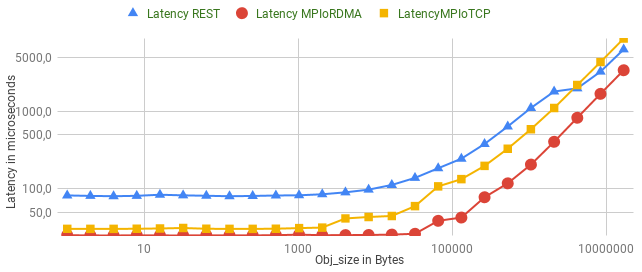
\includegraphics[width=\textwidth]{latency-rest-mpi.png}
\caption{Latency results for the different protocols related to the file size} \label{fig:latency-rest-mpi}
\end{figure}
\begin{figure}
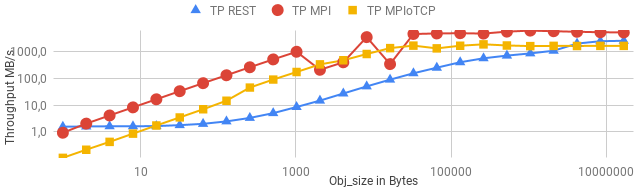
\includegraphics[width=\textwidth]{throughput-rest-mpi.png}
\caption{Throughput results for the different protocols related to the file size} \label{fig:throughput-rest-mpi}
\end{figure}
Our observations and interpretations are as follows:
\begin{itemize}
  \item For small object sizes, the latency of Rest is obviously higher than the one of MPI, as already mentioned in our latency tests, this is due to the HTTP overhead.
  \item The throughput achieved using MPI is better than the one using REST however when comparing MPI and REST both over TCP, we notice that this is not the case especially for very small and large files which leads to the conclusion that the overhead due to the TCP stack is the main factor slowing down the object storage implementation.
  \item The performance dip seen in the red line for a file size of above 1 KB is due to the MPI implementation that uses a combination of protocols for the same MPI routine, namely the use of the eager protocol \cite{eager} for small messages, and rendezvous protocol for larger messages.
\end{itemize}
\begin{figure}
    \centering
    \begin{minipage}{0.49\textwidth}
        \centering
        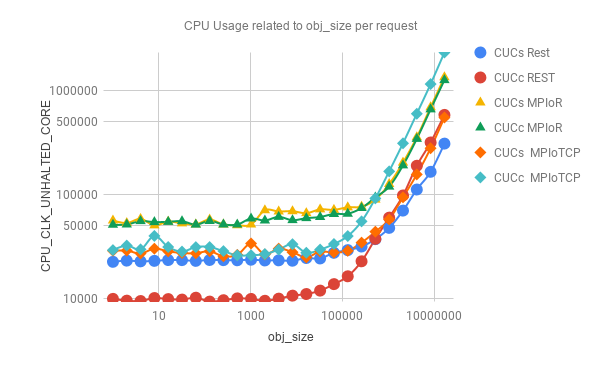
\includegraphics[width=1\textwidth]{cpu-usage-rest-mpi.png}
        \caption{CPU usage per request, on the server and client, for each protocol}
		\label{fig:cpu-usage-rest-mpi}
    \end{minipage}\hfill
    \begin{minipage}{0.49\textwidth}
        \centering
        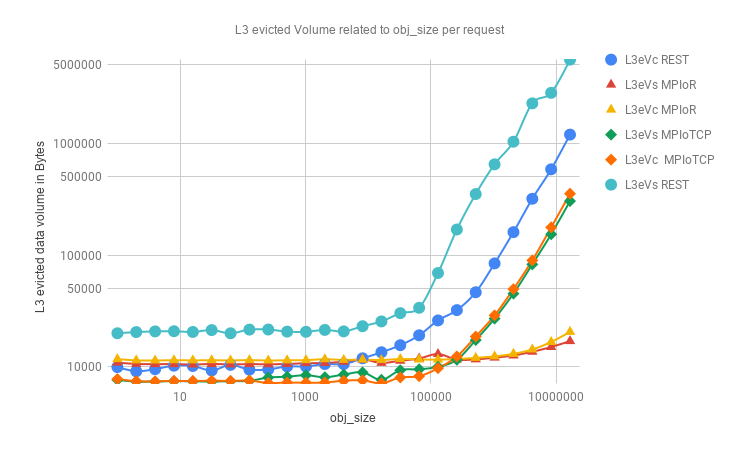
\includegraphics[width=1\textwidth]{l3ev-rest-mpi.png}
        \caption{L3 evicted per request, on the server and client, for each protocol}
		\label{fig:l3ev-rest-mpi}
    \end{minipage}
\end{figure}
\begin{itemize}
\item Another particular finding depicted by \cref{fig:cpu-usage-rest-mpi} is that the CPU cycles needed for the sender to push the data when using MPI is higher than by using REST, this becomes visible for file sizes above 100\,KB.
\item \Cref{fig:l3ev-rest-mpi} shows that, as expected, the evicted data volume stays constant in the case of MPI over RDMAoIB because of the direct data transfer from server main memory to client main memory. Furthermore, the L3-evicted memory for both REST and MPI over TCPoIB is constant for files smaller than 100 KB but increases exponentially afterward. Presumably, because parts of the protocol such as network packets re/assembly is controlled by the kernel and not the network interface.
\end{itemize}

\subsection{HTTP Overhead}

In addition to the overhead and packet fragmentation introduced by the communication protocol in use, TCP in this case, we are interested in the overhead due to the use of HTTP. To calculate the overhead per request, in this case for HTTP 1.1, we have the amount of bytes\_read by the HTTP parser in wrk, and knowing the Number of request achieved, we can assume that:

\[http\_overhead\_per\_byte=\frac{bytes\_read}{Nreq} - obj\-size]\]

We find that the overhead is about 233 bytes for every request, this is due to the uncompressed, literally redundant, HTTP response headers, which can constitute a significant portion of the HTTP traffic, specifically for large numbers of HTTP requests and for files sizes smaller than 1 KB.

\section{Evaluation of the Performance Model} \label{sec:evaluation}
To validate the predictive model defined in \cref{eq:model}, we use the values reported by the REST latency Benchmark on Mistral in \Cref{subsec:tcpib}; the hardware-specific parameters are calculated as follows:

Data between sockets and memory is shipped via a 9.6 GT/s QPI interface \cite{intel-xeon}. According to the Intel QPI specification \cite{intel-qpi} 16 bit of data are transferred per cycle, thus the uni-directional speed is 19,6 GB/s. The communication protocol has an overhead of roughly 11 %, therefore, mem_tp = 17,088 MB/s.
The compute nodes of Mistral are integrated in one FDR InfiniBand fabric, the measured bandwidth between two arbitrary compute nodes is 5.9 GByte/s, as such net\_tp = 5,9 GByte/s, rtt measured using qperf and found = 0.06ms and mtu = 65520 Bytes.

We only need to get the values of the coefficients $\beta_i$ in \cref{eq:model}. This is done by using a regression analysis tool, in this case the one provided by Excel: the obtained R square and F values are examined, for each iteration, to check respectively the fitness and the statistically significant of our model. Finally we calculate the predicted values and we compare them to the ones obtained in the benchmark by determining the error rate using \cref{eq:erro-rate}.

\begin{equation}
 error\%=(t\_req -t\_req\_calcul)\cdot100/t\_req
\label{eq:error-rate}
\end{equation}

In case of RESToTCPoIB, we find that ($\alpha$ = 1) , $\beta_1$ = $\beta_3$ = $\beta_4$ $\sim$ 1 , $\beta_2$ = 6 and $\beta_5$ = 3/2. 
The results are shown in the appendix in Table 1, the deviation (error rate) between the estimated value and the benchmark results is primarily below 10 percent, and indeed in the range of 1 percent for small and large file sizes.\Cref{eq:model} yields:

\begin{equation}
\label{eq:model-rest}
t(request)=rtt+\frac{CUCs}{Rs}+6\cdot\frac{L3EVs}{mem\_tp}+\frac{CUCc}{Rc}+\frac{L3EVc}{mem\_tp}+\frac{3}{2}\cdot\frac{Obj\_size}{net\_tp}
\end{equation}

In case of MPIoTCP, we obtain ($\alpha$ = 0.1), $\beta_1$ = $\beta_2$ = $\beta_3$ = $\beta_4$ $\sim$ 1 , and $\beta_5$ = 2.7. As shown in the appendix in \cref{tab:model-verif-ib}, the deviation (error rate) between the estimated value and the calculated one is primarily below 20 percent, and less than 5 percent for small and large file sizes.
\Cref{eq:model} yields :

\begin{equation}
\label{eq:model-rest}
t(request)=0.1\cdot rtt+\frac{CUCs}{Rs}+\frac{L3EVs}{mem\_tp}+\frac{CUCc}{Rc}+\frac{L3EVc}{mem\_tp}+2.7\cdot\frac{Obj\_size}{net\_tp}
\end{equation}

In case of MPIoRDMA, we obtain ($\alpha$ = 0), $\beta_1$ = $\beta_3$ = 1/2 and  $\beta_2$ = $\beta_4$ = $\beta_5$ $\sim$ 1 . As shown in the appendix in \cref{tab:model-verif-ib}, the deviation (error rate) between the estimated value and the calculated one is primarily below 10 percent, and less than 5 percent for small and large file sizes.
\Cref{eq:model} yields :

\begin{equation}
\label{eq:model-rest}
t(request)=\frac{1}{2}\cdot\frac{CUCs}{Rs}+\frac{L3EVs}{mem\_tp}+\frac{1}{2}\cdot\frac{CUCc}{Rc}+\frac{L3EVc}{mem\_tp}+\frac{Obj\_size}{net\_tp}
\end{equation}

By investigating the model terms, we can infer some general behavior and verify our expectations. The latency for MPIoRDMA is expected to be lower than the others, this  is why $\alpha$ is close to 0 for this model. If $\beta_5$ is above 1, it is an indicator that we cannot achieve full network throughput. REST and MPIoTCP show otherwise similar performance characteristics while the MPIoRDMA model is approximated to use half the CUC, which actually means it needed twice as many compared to the TCP models - maybe due to busy waiting. These assumptions can be verified by looking at \Cref{fig:cpu-usage-rest-mpi} and \Cref{fig:l3ev-rest-mpi}.

In conclusion, we notice that while TCP proved itself for end-to-end communications over long distances, it is however less suitable for data center networking, mainly because of its processing overhead (CPU and memory resources consumption), hence degrading the aspired performance. On the other side, CPU and Memory consumption for the REST over TCP Model remained adequate in comparison with MPI over TCP and MPI over RDMA.


\subsection{Comparing the different protocols: HTTP1.1 vs HTTP2 vs HTTP3}


The latency and throughput results of the tests on the WR cluster are shown in Fig.14 and Fig.15 respectively:





Based on the defined model, we compare the performance of the different HTTP protocols, the same setup described in \cref{fig:wrk2bench} is used here, however the web server, in this case, should be able to deliver the three different protocols. Therefore, openlitespeed \cite{openlitespeed} is used and the suitable benchmark tool is h2load \cite{h2load}.


To note that we test here the ngtcp2 \cite{ngtcp2} implementation of HTTP3, because it's TLS library independent, not like other HTTP3 implementations like quiche \cite{quiche} which requires boringssl. Since at the time of writing, the official OpenSSL Team doesn’t support QUIC \cite{opensslquicblog} we use a patched version of OpenSSL provided by the ngtcp2 team.
Since HTTP3 didn't achieve the maturity phase yet, we are using the protocols as they are defined in the 27th Draft by the IETF QUIC Working group \cite{quicwg}.

The latency and throughput results of the tests on the WR cluster are shown in \Cref{fig:lat-comp} and \Cref{fig:rps-comp} respectively:

\begin{figure}[H]
    \centering
    \begin{minipage}{0.49\textwidth}
        \centering
        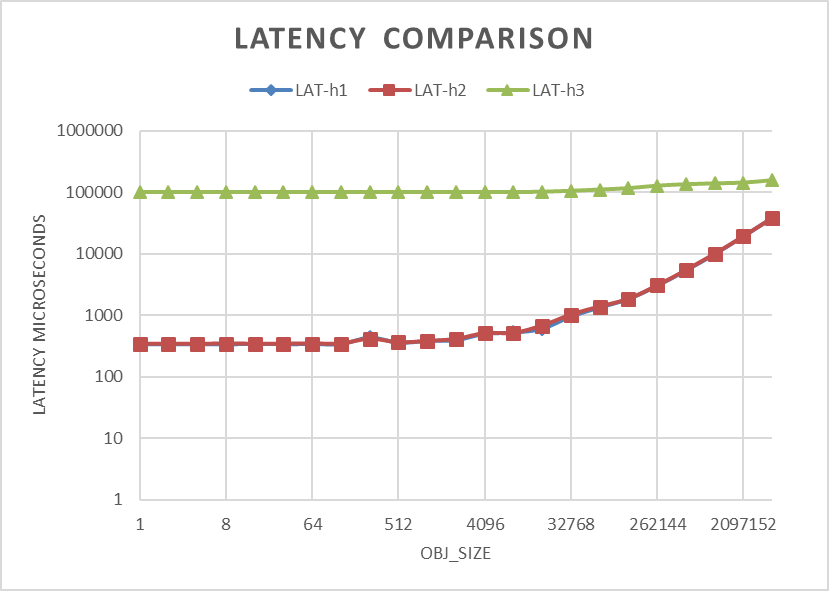
\includegraphics[width=1\textwidth]{lat-comparison-h2load.png}
        \caption{Latency results for the different protocols}
		\label {fig:lat-comp}
    \end{minipage}\hfill
    \begin{minipage}{0.49\textwidth}
        \centering
        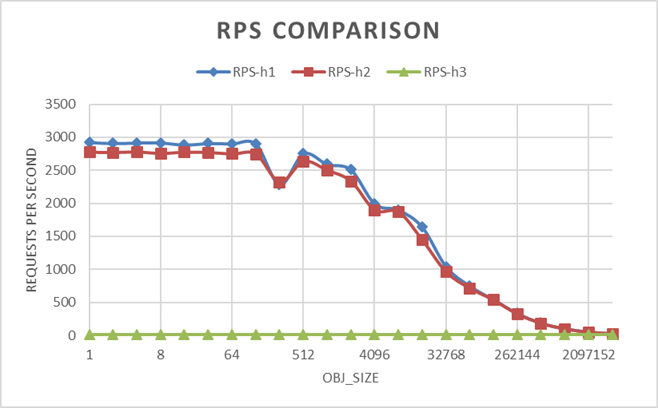
\includegraphics[width=1\textwidth]{rps-comparison-h2load.png}
        \caption{Throughput results for the different protocols}
		\label {fig:rps-comp}
    \end{minipage}
\end{figure}

Similar results were also obtained on Mistral over InfiniBand:

\begin{figure}[H]
    \centering
    \begin{minipage}{0.49\textwidth}
        \centering
        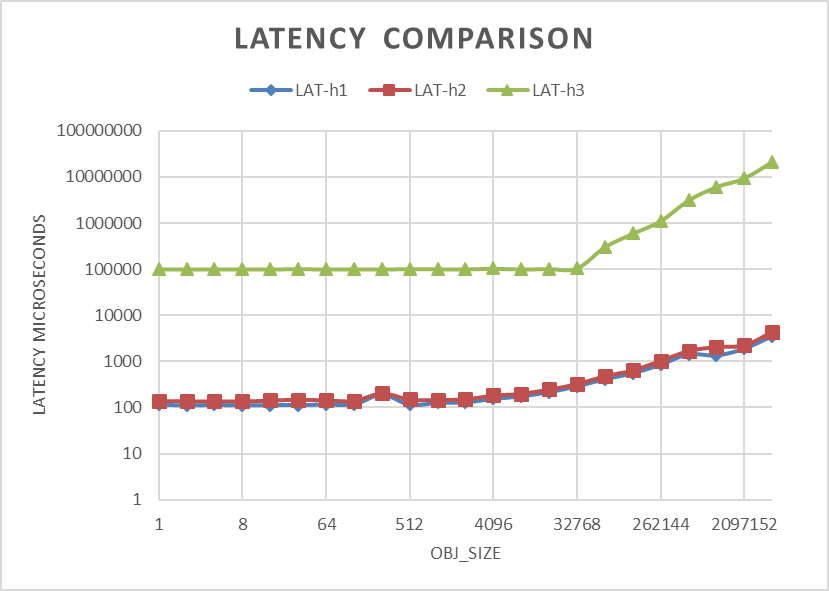
\includegraphics[width=1\textwidth]{lat-h2load-mistral.png}
        \caption{Latency results for the different protocols}
		\label {fig:lat-comp-mistral}
    \end{minipage}\hfill
    \begin{minipage}{0.49\textwidth}
        \centering
        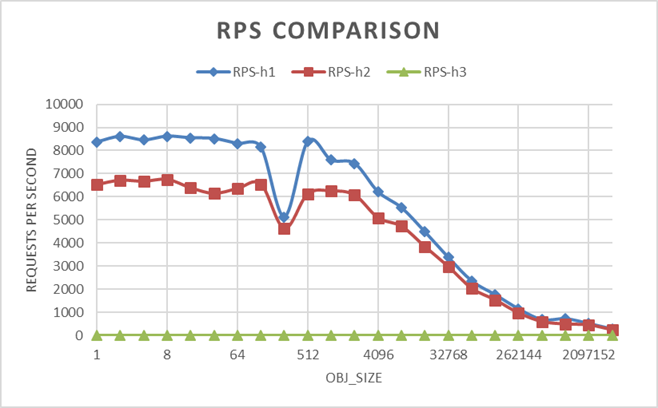
\includegraphics[width=1\textwidth]{rps-h2load-mistral.png}
        \caption{Throughput results for the different protocols}
		\label {fig:rps-comp-mistral}
    \end{minipage}
\end{figure}


Although we are expecting HTTP2 and HTTP3 to perform better than HTTP 1.1, this is not the case. A closer look at the evolution of the parameters defined in our model reveals the cause:

\begin{figure}[H]
    \centering
    \begin{minipage}{0.49\textwidth}
        \centering
        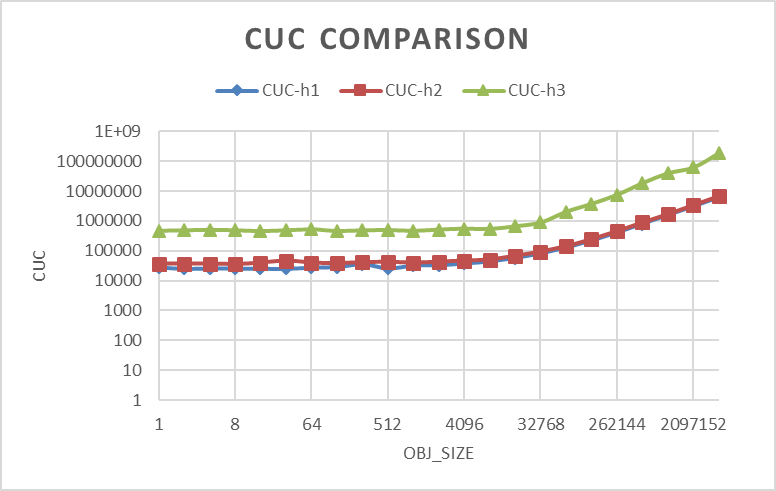
\includegraphics[width=1\textwidth]{cuc-h2load-mistral.png}
        \caption{Client CPU Consumption for the different protocols}
		\label {fig:cuc-comp}
    \end{minipage}\hfill
    \begin{minipage}{0.49\textwidth}
        \centering
        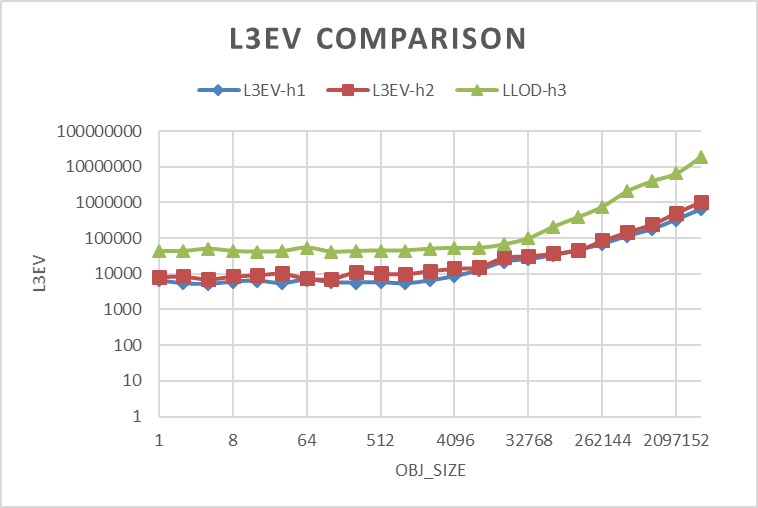
\includegraphics[width=1\textwidth]{l3ev-h2load-mistral.png}
        \caption{Client Memory consumption for the different protocols}
		\label {fig:llod-comp}
    \end{minipage}
\end{figure}


Despite the obvious traffic saving of HTTP2, it comes at a considerable memory consumption, which renders the gained advantages negligible. The chosen HTTP3 implementation is circa 10 times CPU and memory consuming in comparison to the earlier versions, which indicates an implementation issue.

\section{Summary}

This paper provides a first assessment of using REST as a storage protocol in an HPC environment. A performance model for the relevant HTTP Get/Put operation based on hardware counters is provided and experimentally validated. Our results demonstrate that, when the same transport protocol is in use, i.e. TCP, REST can provide similar latency and throughput to the HPC-specific interface MPI while enabling better portability.
A careful comparison of the different HTTP Protocols suggests that the new techniques introduced by the newer versions of the protocol -- like the use of a small number of connections, multiplexing the HTTP datagram, compressing the header and allowing the server to “push” data pro-actively to the client whilst eventually using UDP to accomplish these -- bear the potential to improve performance and, thus, provide a perspective for using cloud storage inside HPC environments.
As future work, we aim to validate that REST is a performant and efficient alternative to common HPC I/O protocols in an actual HPC scenario.

\section{Appendix}

Tables can be found at : \href{https://github.com/http-3/rest-overhead-paper}{https://github.com/http-3/rest-overhead-paper}.




\nocite{*}
%
% ---- Bibliography ----
%
% BibTeX users should specify bibliography style 'splncs04'.
% References will then be sorted and formatted in the correct style.
%



\bibliographystyle{splncs04}
\bibliography{biblio}


\end{document}
